% !TeX spellcheck = ru_RU-Russian
\section{Рабочий проект}
\subsection{Классы, используемые при разработке программы}

\subsubsection{Класс Test}

Данный класс необходим для проведения тестирования. Для создания объекта требуется передать название теста и список вопросов. Методы класса описаны в таблице \ref{test_functions:table}. Свойства класса описаны в таблице \ref{test_properties:table}

\begin{xltabular}{\textwidth}{|p{6cm}|X|}
	\caption{Таблица методов класса Test\label{test_functions:table}} \hline
	\centrow Метод & \centrow Описание метода \\ \hline
	\endfirsthead
	\continuecaption{Продолжение таблицы \ref{test_functions:table}}  \hline
	\centrow Метод & \centrow Описание метода \\ \hline
	\finishhead
	print\_current\_question(self) & Возвращает номер вопроса и текст вопроса в виде строки "<№\{Номер вопроса\}. \{Текст вопроса\}">. \\ \hline
	shuffle\_questions(self) & Перемешивает вопросы текущего теста случайным образом, ничего не возвращает. \\ \hline
	shuffle\_answers(self) & Перемешивает ответы текущего вопроса, ничего не возвращает. \\ \hline
	start\_test(self) & Запускает тест, обнуляет счёт и устанавливает id текущего вопроса, ничего не возвращает. \\ \hline
	next\_question(self) & Выполняет инкремент id текущего вопроса и перемешивает его ответы, ничего не возвращает. \\ \hline
	accept\_answers(self, user\_answers: List[Answer]) & Проверяет ответ на базовый вопрос и увеличивает счёт, если ответ правильный. Ничего не возвращает. \\ \hline
	\_increase\_score(self) & Увеличивает счёт, ничего не возвращает. \\ \hline
	calculate\_right\_answers\_ percentage(questions\_count, right\_answers\_count) & Статический метод. Принимает количество всех вопросов  и количесвто правильных вопросов. Расчитывает отношение правильных ответов к количеству вопросов возвращает процентное соотношение. \\ \hline
	summarise(self) & Возвращает процентное соотношение правильных ответов к общему количеству вопросов.
\end{xltabular}

\begin{xltabular}{\textwidth}{|p{6cm}|X|}
	\caption{Таблица свойств класса Test\label{test_properties:table}} \hline
	\centrow Свойство & \centrow Описание свойства \\ \hline
	\endfirsthead
	\continuecaption{Продолжение таблицы \ref{test_properties:table}}  \hline
	\centrow Свойство & \centrow Описание свойства \\ \hline
	\finishhead
	questions\_count(self) & Возвращает количество вопросов. \\ \hline
	get\_current\_question(self) & Возвращает текущий вопрос. \\ \hline
	get\_current\_answers(self) & Возвращает ответы текущего вопроса. \\ \hline
	is\_finished(self) & Возвращает статус завершения теста.
\end{xltabular}

\subsubsection{Класс FileProvider}

Данный класс статический, и используется другими классами для работы с файловой системой. Методы класса описаны в таблице \ref{fileProvider_functions:table}.

\begin{xltabular}{\textwidth}{|p{6cm}|X|}
	\caption{Таблица методов класса QuestionsStorage\label{fileProvider_functions:table}} \hline
	\centrow Метод & \centrow Описание метода \\ \hline
	\endfirsthead
	\continuecaption{Продолжение таблицы \ref{fileProvider_functions:table}} 
	\centrow Метод & \centrow Описание метода \\ \hline
	\finishhead
	get\_admin\_password() & Обращается к файлу, содержащему пароль администратора, извлекает данные, десерилизует их и возвращает пароль администратора. \\ \hline 
	set\_admin\_ password(new\_password) & Принимает новый пароль администратора, обращается к файлу, содержащему пароль администратора, сериализует новый пароль и перезаписывает старый пароль на новый. Если файла не существует, создаёт его. Ничего не возвращает. \\ \hline
	save\_user(user: User) & Принимает объект класса User(пользователь), сериализует данные пользователя и сохраняет в файл, содержащий информацию о пользователях. Если файла не существует, создаёт его. Ничего не возвращает. \\ \hline
	delete\_user(user\_name: str) & Принимает имя пользователя. Находит в файле, содержащем информацию о пользователях, пользователя с переданным именем и удаляет его. Ничего не возвращает. \\ \hline
	get\_users() & Извлекает и десериализует данные о пользователях из соответствующего файла. Возвращает список пользователей. \\ \hline
	save\_test\_result(test\_result: TestResult) & Принимает объект класса TestResult, сериализует его и сохраняет в файл с результатами. Если файла не существует, создаёт его. Ничего не возвращает. \\ \hline
	get\_results() & Извлекает и десериализует результаты прохождения тестов всех пользователей. Возвращает список результатов. \\ \hline
	clear\_test\_results() & Удаляет файл результатов. \\ \hline
	save\_test(test: Test) & Принимает объект класса Test, сериализует его и сохраняет в файл с тестами. Если файла не существует, создаёт его. Ничего не возвращает. \\ \hline
	get\_test(test\_path: str) & Принимает путь к тесту, извлекает данные теста и десериализует их. Возвращает объект класса Test. \\ \hline
	save\_test\_changes(test: Test, test\_path: str) & Принимает объект класса Test и путь для его сохранения. Сериализует данные теста, создаёт файл с именем теста и сохраняет в него данные. Ничего не возвращает. \\ \hline
	get\_test\_names() & Находит все существующие тесты в папке "<Tests">. Возвращает список их названий найденных тестов. \\ \hline
	find\_test\_path(wanted\_test \_name: str) & Принимает имя искомого теста. Находит путь к тесту с данным именем. Возвращает строку - путь к искомому тесту.
\end{xltabular}

\subsubsection{Класс QuestionsStorage}

Данный класс характеризует хранилище вопросов, позволяет добавлять вопрос, удалять вопрос, обновлять список вопросов и сохранять изменения. Для работы с файлами использует методы статического класса FileProvider, который описан выше. Методы класса QuestionsStorage описаны в таблице \ref{questionsStorage_functions:table}.

\begin{xltabular}{\textwidth}{|p{6cm}|X|}
	\caption{Таблица методов класса QuestionsStorage\label{questionsStorage_functions:table}} \hline
	\centrow Метод & \centrow Описание метода \\ \hline
	\endfirsthead
	\continuecaption{Продолжение таблицы \ref{questionsStorage_functions:table}} 
	\centrow Метод & \centrow Описание метода \\ \hline
	\finishhead
	add\_question(self, question) & Добавляет вопрос в хранилище. \\ \hline 
	remove\_question(self, question\_number) & Принимает индекс вопроса. Удаляет вопрос по индексу из хранилища. \\ \hline
	update\_test(self, test\_path: str) & Принимает строку - путь к файлу с вопросами. Обновляет текущий список вопросов из файла по переданному пути. Ничего не возвращает. \\ \hline
	save\_changes(self) & Сохраняет изменения по пути текущего теста. Ничего не возвращает.
\end{xltabular}

\subsubsection{Класс Validation}

Данный класс содержит методы для проверки ввода пользователя. Методы класса Validation описаны в таблице \ref{validation_functions:table}.

\begin{xltabular}{\textwidth}{|p{6cm}|X|}
	\caption{Таблица методов класса QuestionsStorage\label{validation_functions:table}} \hline
	\centrow Метод & \centrow Описание метода \\ \hline
	\endfirsthead
	\continuecaption{Продолжение таблицы \ref{validation_functions:table}} 
	\centrow Метод & \centrow Описание метода \\ \hline
	\finishhead
	validate\_user\_name (username: str) & Принимает и проверяет имя пользователя. Возвращает True, если имя не слишком короткое, иначе - False. \\ \hline 
	check\_name\_ uniqueness(username) & Принимает и проверяет уникальность имени пользователя. Возвращает True, если имя уникально и не было найдено среди зарегистрированных пользователей, иначе возвращает False. \\ \hline
	validate\_question(question) & Принимает и проверяет строку - текст вопроса. Возвращает True, если количество символов вопроса не меньше 4 и не больше 120, иначе возвращает False. \\ \hline
	validate\_answer(answer) & Принимает и проверяет строку - ответ на вопрос. Возвращает True, если строка не пустая, иначе возвращает False
\end{xltabular}
\newpage

\subsection{Модульное тестирование разработанного приложения}

На рисунке \ref{unitTestValidation_code:image} представлен код модульного тестирования класса "<Validation">.

\begin{figure}[H]
\begin{lstlisting}[language=Python]
import unittest
import validation
from validation import Validation


class TestValidation(unittest.TestCase):
	def test_validate_user_name(self):
		correct_user_name = "Fedor"
		self.assertTrue(Validation.validate_user_name(correct_user_name))
		incorrect_user_name = "F"
		self.assertFalse(Validation.validate_user_name(incorrect_user_name))
		with self.assertRaises(TypeError):
			Validation.validate_user_name(1)

	def test_check_name_uniqueness(self):
		correct_user_name = "Евлампий Евстрахович"
		self.assertTrue(Validation.check_name_uniqueness(correct_user_name))
		incorrect_user_name = "Администратор"
		self.assertFalse(Validation.check_name_uniqueness(incorrect_user_name))
			with self.assertRaises(TypeError):
				Validation.check_name_uniqueness(21)

	def test_validate_question(self):
		correct_question = "Сколько будет 2+2*2?"
		self.assertTrue(Validation.validate_question(correct_question))
		incorrect_question = "33?"
		self.assertFalse(Validation.validate_question(incorrect_question))
			with self.assertRaises(TypeError):
				Validation.validate_question(321)

	def test_validate_answer(self):
		correct_answer = "6"
		self.assertTrue(Validation.validate_answer(correct_answer))
		incorrect_answer = ""
		self.assertFalse(Validation.validate_answer(incorrect_answer))
			with self.assertRaises(TypeError):
				Validation.validate_answer(4315)

if __name__ == "__main__":
unittest.main()
\end{lstlisting}  
\caption{Код модульного теста класса "<Validation">}
\label{unitTestValidation_code:image}
\end{figure}

Результат тестирования класса "<Validation"> представлен на рисунке \ref{unitTest_validation_result:image}

\begin{figure}[ht]
	\centering
	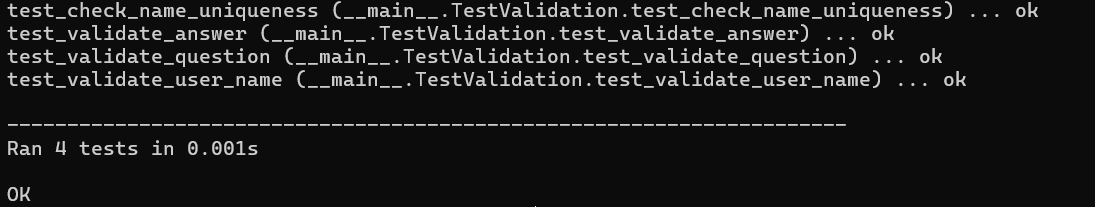
\includegraphics[width=1\linewidth]{unitTest_validation.png}
	\caption{Результат модульного тестирования класса "<Validation">}
	\label{unitTest_validation_result:image}
\end{figure}

\subsection{Системное тестирование разработанного приложения}


